\documentclass[a4paper]{article}
\usepackage{cmap}
\usepackage[utf8]{inputenc}
\usepackage[russian]{babel}
\usepackage{float}
\usepackage{graphicx}
\usepackage{amsmath}
\usepackage{amssymb}
\usepackage{amsthm}
\usepackage[unicode, pdfborder = {0 0 0}, colorlinks, urlcolor = black, linkcolor = black, citecolor = black]{hyperref}
\usepackage[raggedright]{titlesec}
\usepackage{mathtools}
\usepackage{pgfplots}
\usepackage{multirow}
\usepackage{comment}
\usepackage{indentfirst}  % Для отступа в первом абзаце каждой главы
\usepackage[skip=0pt]{caption}
\usepackage{etoolbox}
\usepackage{listings} % для поддержки синтаксиса Python


\patchcmd{\thebibliography}{\section*{\refname}}{}{}{} % Для нумерации библиографии

\DeclarePairedDelimiter\ceil{\lceil}{\rceil}
\DeclarePairedDelimiter\floor{\lfloor}{\rfloor}

\titleformat{\chapter}[block]
{\normalfont\huge\bfseries}{\thechapter}{20pt}{}
\titlespacing*{\chapter}
{0pt}{20pt}{20pt}

\setcounter{tocdepth}{5}
\setcounter{secnumdepth}{5}
\setcounter{MaxMatrixCols}{20}

\parindent = 7mm
\oddsidemargin = 5mm
\topmargin = -10mm
\textheight = 240mm
\textwidth = 165mm
\linespread{1.5}
\pgfplotsset{compat=1.15}

\renewcommand{\small}{\fontsize{12}{14.5pt}\selectfont}
\renewcommand{\normalsize}{\fontsize{14}{16pt}\selectfont}
\renewcommand{\large}{\fontsize{17}{20pt}\selectfont}
\renewcommand{\Large}{\fontsize{20}{25pt}\selectfont}
\renewcommand{\LARGE}{\fontsize{25}{30pt}\selectfont}
\renewcommand\qedsymbol{$\blacksquare$}

\newtheorem{theorem}{Теорема}[section]
\theoremstyle{definition}
\newtheorem{statement}{Утверждение}[section]
\newtheorem{definition}{Определение}[section]
\newtheorem*{example}{Пример}

\newenvironment{Proof}
{{\bf \flushleft{Доказательство.} \\}}
{\hfill$\scriptstyle\blacksquare$}

\newcounter{qcounter}

\begin{document}

\normalsize

\thispagestyle{empty}
\begin{titlepage}
\begin{center}

\vfill
МИНОБРНАУКИ РОССИИ\\
\vspace*{0.3cm}
Федеральное государственное автономное образовательное\\
учреждение высшего образования\\
«Южный федеральный университет»\\
\vspace*{0.3cm}
Институт математики, механики и компьютерных наук им.\\
И.И.Воровича\\
Кафедра алгебры и дискретной математики
\vfill

\bigskip

{\large\bf Архипов~Антон~Евгеньевич}
\vfill
{\large\bf РЕАЛИЗАЦИЯ НЕЙРОННОЙ СЕТИ, ВЫПОЛНЯЮЩЕЙ ДЕКОДИРОВАНИЕ КОДА ХЭММИНГА С ИСПОЛЬЗОВАНИЕМ ТЕХНОЛОГИИ GOOGLE COLABORATORY}

\fontsize{14}{16pt}\selectfont

\vfill
ВЫПУСКНАЯ КВАЛИФИКАЦИОННАЯ\\ РАБОТА БАКАЛАВРА\\
по направлению 01.03.02 — Прикладная математика и информатика
\vfill

{\bf Научный руководитель~---\\
к.т.н.~Мкртичян Вячеслав Виталиевич}

\vfill

\end{center}

\bigskip

\begin{center}
Ростов-на-Дону~---~2018
\end{center}

\end{titlepage} 

\tableofcontents
\newpage

\section{Введение}
%\addcontentsline{toc}{section}{Введение}

В~последние годы методы глубокого обучения продемонстрировали значительные улучшения в~различных задачах\cite{bib:buhrstein}. Эти методы превосходят человека в~решении задачи обнаружения объектов и позволяют достичь самых высоких результатов в~области машинного перевода и обработки речи. Кроме того, глубокое обучение в~сочетании с~методом обучения с~подкреплением выигрывают партии у~чемпионов в~сложных играх, например в~Го\cite[c.\,484–489]{bib:win_go}.

Помехоустойчивые коды\cite[с.\,4]{bib:codes} используются для~установки надежного соединения и позволяют обмениваться информацией и исправлять ошибки, полученные в~результате передачи данных по каналу связи. Они применяются в магнитных и оптических системах хранения информации, системах цифровой связи, в том числе: спутниковой, сотовой, передаче данных по телефонным каналам. Очевидно, что полезность помехоустойчивых кодов крайне велика для всего человечества, так как появление ошибки в базе данных какого-нибудь банка может привести как к экономическим, так и юридическим конфликтам. Одним~из~примеров такого кода является код~Хэмминга\cite[с.\,49]{bib:codes2}. За~счет добавления к~информационному слову избыточности, он~позволяет исправлять одну ошибку. Декодирование\cite[c.\,5]{bib:codes} кода можно представить в~виде некоторой функции. Согласно универсальной теореме аппроксимации\cite{bib:approximation_theorem} нейронная сеть\cite[с.\,23]{bib:neural_networks} может аппроксимировать непрерывную функцию многих переменных с~любой точностью.

В~данной работе представлено исследование возможности аппроксимации нейронной сетью $\mathcal{N}$ функции декодирования кода Хэмминга~(16,~11). Прямым подходом к~решению задачи декодирования кода Хэмминга нейронной сетью является обучение модели на~наборе данных, состоящем из большого количества кодовых слов с~добавлением ошибки в~случайно выбранной позиции.


\newpage 

\section{Необходимые сведения}
%\addcontentsline{toc}{section}{Необходимые сведения}

\subsection{Нейронные сети}\label{subsec:neural_network}
%\addcontentsline{toc}{subsection}{Нейронные сети}

\begin{definition}
  Искусственная нейронная сеть (нейронная сеть)~---~математическая модель, а~также её программная реализация, построенная по~принципу организации и функционирования биологических нейронных сетей.
\end{definition}
Это понятие возникло при~изучении процессов, протекающих в~мозге, и при~попытке смоделировать их. После разработки алгоритмов обучения получаемые модели стали использовать в~практических целях: в~задачах прогнозирования, для~распознавания образов, в~задачах управления и др.
Нейронная сеть представляет собой систему соединённых и взаимодействующих между собой простых процессоров (искусственных нейронов).
Каждый процессор подобной сети имеет дело только с~сигналами, которые он получает, и сигналами, которые он периодически посылает другим процессорам. И, тем~не~менее, будучи соединёнными в~достаточно большую сеть с~управляемым взаимодействием, такие по~отдельности простые процессоры вместе способны выполнять сложные задачи.

Нейронные сети не программируются в~привычном смысле этого слова, они обучаются. Возможность обучения~--~одно из~главных преимуществ нейронных сетей перед традиционными алгоритмами. Технически обучение заключается в~нахождении коэффициентов связей между нейронами. В~процессе обучения нейронная сеть способна выявлять сложные зависимости между входными данными и выходными, а~также выполнять обобщение. Это значит, что в~случае успешного обучения сеть сможет вернуть верный результат на~основании данных, которые отсутствовали в~обучающей выборке, а~также неполных и/или «зашумленных», частично искажённых данных.

\begin{figure}[h]
    \centering
    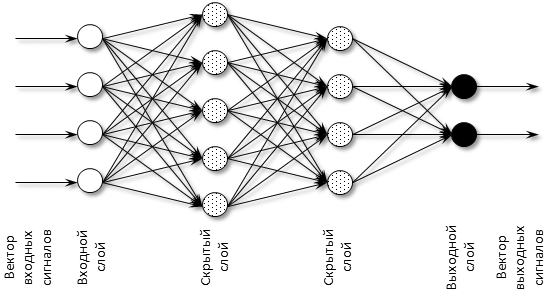
\includegraphics[width=0.8\textwidth]{nn_vizualisation}
    \caption{Полносвязная нейронная сеть.}
    \label{fig:nn}
\end{figure}

Обучение полносвязной\cite[с.\,44]{bib:neural_networks} нейронной сети с~$L$ скрытыми слоями\cite[с.\,43]{bib:neural_networks} происходит в несколько этапов. Для каждого вектора из набора данных выполняются следующие операции:
\begin{enumerate}\label{alg:neural_education}
\item Вектор входных параметров $x_0$ передается на входной слой~$l_0$ нейронной сети.
\item От каждого нейрона входного слоя значения передаются к каждому из $K_1$ нейронов первого скрытого слоя $l_1$ нейронной сети.
\item Каждый нейрон скрытого слоя вычисляет скалярное произведение \newline $y~=~\langle~W_i, x_{i-1}~\rangle$, где $i\in\{1; \dots; L\}$~-~номер текущего слоя, $W_i$~-~вектор весов $i$-го слоя, а $x_{i-1}$~-~вектор значений, полученных с $(i-1)$-го слоя.
\item Вычисляется выходное значение нейрона $x_i = f_{a_i}(y)$, где $f_{a_i}$~-~функция активации\cite[с.\,151]{bib:neural_networks2} $i$-го слоя.
\item Выходное значение $x_i$ передается каждому из $K_{i+1}$ нейронов следющего слоя. Если следующий слой не~является выходным, то~повторяются шаги (3)-(4), иначе полученный вектор выходных значений~$x_{L+1}$ является ответом нейронной сети.
\end{enumerate}

\newpage

Далее, векторы $x_{L+1}$, полученные для~каждого элемента из~набора данных, сравниваются по~заданной метрике\cite{bib:metrics} $\rho$ с~ответами
и вычислятся значение функции потерь\cite[с.\,65]{bib:neural_networks2} $f_{loss}$. После чего веса $W_i$ для $i\in\{1; \dots; L\}$ пересчитываются по~методу обратного распространения ошибки\cite[с.\,151-184]{bib:neural_networks2} и алгоритм повторяется.

Таким образом, нейронная сеть задается следующими параметрами: количество скрытых слоев $L$, функция активации $f_{a,i}$ и количество нейронов $K_i$ для $i\in\{1; \dots; L\}$, функция потерь $f_{loss}$ и метрика $\rho$.

%\newpage 

\subsection{Код Хэмминга}
%\addcontentsline{toc}{subsection}{Код Хэмминга}

Целью данной работы является построение декодера на основе нейронной сети. Для её обучения требуется достаточный набор данных. Код Хэмминга $\mathbb{C}(n,k)$, $n = 16, k = 11$, подходит для обучения, так как пространство его информационных слов достаточно для~обучения нейронной сети.

Порождающая матрица $G$ имеет вид:
\begin{equation}
G =
\begin{pmatrix}
0 & 0 & 0 & 0 & 0 & 0 & 0 & 0 & 1 & 0 & 0 & 1 & 1 & 0 & 1 & 0 \\
0 & 0 & 0 & 0 & 0 & 0 & 1 & 0 & 0 & 0 & 0 & 0 & 1 & 0 & 1 & 1 \\
0 & 0 & 0 & 0 & 0 & 1 & 0 & 0 & 0 & 0 & 0 & 0 & 1 & 1 & 0 & 1 \\
0 & 0 & 0 & 0 & 1 & 0 & 0 & 0 & 0 & 0 & 0 & 0 & 1 & 1 & 1 & 0 \\
0 & 0 & 0 & 1 & 0 & 0 & 0 & 0 & 0 & 0 & 0 & 1 & 0 & 0 & 1 & 1 \\
0 & 0 & 1 & 0 & 0 & 0 & 0 & 0 & 0 & 0 & 0 & 1 & 0 & 1 & 0 & 1 \\
0 & 1 & 0 & 0 & 0 & 0 & 0 & 0 & 0 & 0 & 0 & 1 & 0 & 1 & 1 & 0 \\
1 & 0 & 0 & 0 & 0 & 0 & 0 & 0 & 0 & 0 & 0 & 1 & 1 & 0 & 0 & 1 \\
0 & 0 & 0 & 0 & 0 & 0 & 0 & 1 & 0 & 0 & 0 & 0 & 0 & 1 & 1 & 1 \\
0 & 0 & 0 & 0 & 0 & 0 & 0 & 0 & 0 & 1 & 0 & 1 & 1 & 1 & 0 & 0 \\
0 & 0 & 0 & 0 & 0 & 0 & 0 & 0 & 0 & 0 & 1 & 1 & 1 & 1 & 1 & 1
\end{pmatrix}
\end{equation}

Пусть $L = 2^k$. Кодирование информационных слов из $\mathbb{F}_2^L$ в код $\mathbb{C}$ осуществляется путем умножения на матрицу $G$.
Процесс кодирования заключается в~умножении информационного слова на~данную матрицу.

На практике доказано, что при~систематическом виде нейронная сеть вырождается в~тождественный оператор. Именно этим обусловлен выбор такой порождающей матрицы.

Проверочные биты записываются в~конец информационного слова. Для нейронной сети не~имеет значения, находятся ли~проверочные биты целиком в~конце или на~определенных позициях слова.
%\newpage
Для~проверки корректного информационных слов на наличие ошибок используется соответствующая проверочная матрица.

\begin{equation}
H =
\begin{pmatrix}
1 & 1 & 1 & 1 & 0 & 0 & 0 & 0 & 1 & 1 & 1 & 1 & 0 & 0 & 0 & 0 \\
1 & 0 & 0 & 0 & 1 & 1 & 1 & 0 & 1 & 1 & 1 & 0 & 1 & 0 & 0 & 0 \\
0 & 1 & 1 & 0 & 1 & 1 & 0 & 1 & 0 & 1 & 1 & 0 & 0 & 1 & 0 & 0 \\
0 & 1 & 0 & 1 & 1 & 0 & 1 & 1 & 1 & 0 & 1 & 0 & 0 & 0 & 1 & 0 \\
1 & 0 & 1 & 1 & 0 & 1 & 1 & 1 & 0 & 0 & 1 & 0 & 0 & 0 & 0 & 1
\end{pmatrix}
\end{equation}

При~таких параметрах данный код позволяет гарантированно исправлять одну ошибку.

%   \newpage 

\section{Google Colaboratory}\label{section:google_colab}

\textbf{Python}\cite{bib:python}~-~высокоуровневый, интерпретируемый язык программирования общего назначения с открытым исходным кодом.
Выбор данного языка обусловлен большим количеством высокоуровневых библиотек, позволяющих проводить исследования в~области машинного обучения и нейронных сетей.
Большое сообщество разработчиков на языке Python позволяет находить ответы на возникающие вопросы\cite{bib:why_python}.

\textbf{Jupyter Notebook}\cite{bib:jupyter}~-~веб-приложение, позволяющее создавать документы, содержащие программный код, визуализацию и текст.

% ссылка на статью с настройками
\textbf{Google Colaboratory}\cite{bib:colab_settings}~-~бесплатный исследовательский инструмент для машинного обучения.
Это оболочка Jupyter Notebook позволяющая проводить все вычисления на~удаленном сервере на~видеокарте NVIDIA Tesla K80\cite{bib:nvidia_k80}, не~требуя наличия высокопроизводительного оборудования.

\newpage

Для начала работы необходимо выполнить следующие действия:
\begin{enumerate}\label{alg:colab_settings}
\item Создать документ Colaboratory
\begin{figure}[h]
    \centering
    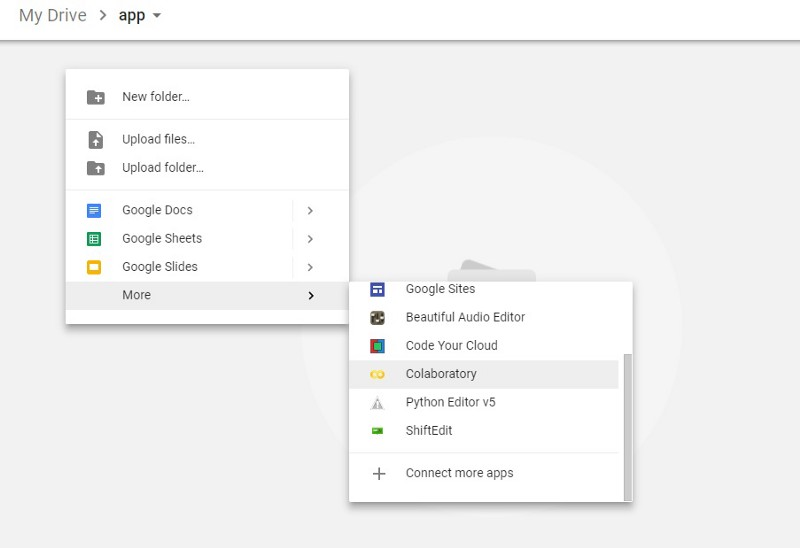
\includegraphics[width=0.8\textwidth]{colab_settings_1.jpeg}
    \label{fig:colab_settings_1}
\end{figure}

\item В разделе \textsl{Runtime->Change runtime type} выбрать GPU
\begin{figure}[h]
    \centering
    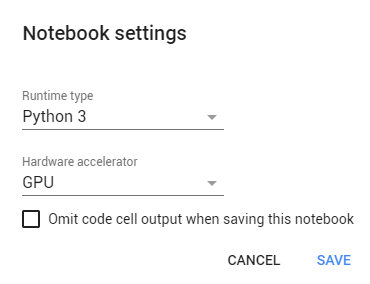
\includegraphics[width=0.6\textwidth]{colab_settings_2.png}
    \label{fig:colab_settings_2}
\end{figure}

\newpage

\item На данном этапе уже можно использовать Google Colaboratory
\begin{figure}[h]
    \centering
    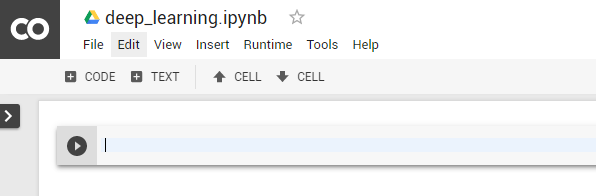
\includegraphics[width=0.85\textwidth]{colab_settings_3.png}
    \label{fig:colab_settings_3}
\end{figure}

\item Авторизуем учетную запись Google и подключим Google Drive следующими командами
\begin{figure}[h]
    \centering
    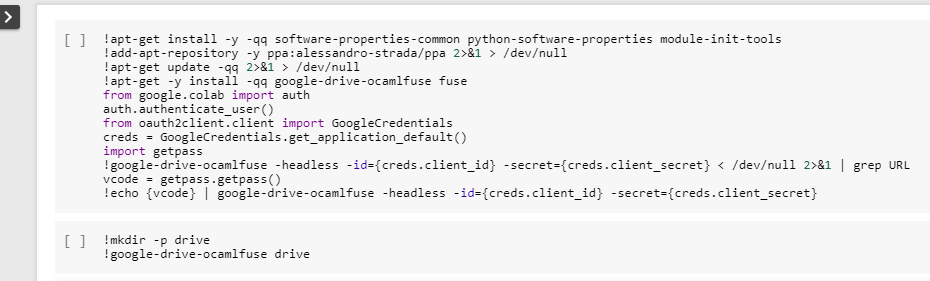
\includegraphics[width=0.85\textwidth]{colab_settings_4.png}
    \label{fig:colab_settings_4}
\end{figure}

\end{enumerate}

Теперь можно производить вычисления нa видеокарте NVIDIA Tesla K80 и взаимодействовать с Google Drive.

\newpage 

\newpage 

\section{Google Colaboratory}\label{section:google_colab}

\textbf{Python}\cite{bib:python}~-~высокоуровневый, интерпретируемый язык программирования общего назначения с открытым исходным кодом.
Выбор данного языка обусловлен большим количеством высокоуровневых библиотек, позволяющих проводить исследования в~области машинного обучения и нейронных сетей.
Большое сообщество разработчиков на языке Python позволяет находить ответы на возникающие вопросы\cite{bib:why_python}.

\textbf{Jupyter Notebook}\cite{bib:jupyter}~-~веб-приложение, позволяющее создавать документы, содержащие программный код, визуализацию и текст.

% ссылка на статью с настройками
\textbf{Google Colaboratory}\cite{bib:colab_settings}~-~бесплатный исследовательский инструмент для машинного обучения.
Это оболочка Jupyter Notebook позволяющая проводить все вычисления на~удаленном сервере на~видеокарте NVIDIA Tesla K80\cite{bib:nvidia_k80}, не~требуя наличия высокопроизводительного оборудования.

\newpage

Для начала работы необходимо выполнить следующие действия:
\begin{enumerate}\label{alg:colab_settings}
\item Создать документ Colaboratory
\begin{figure}[h]
    \centering
    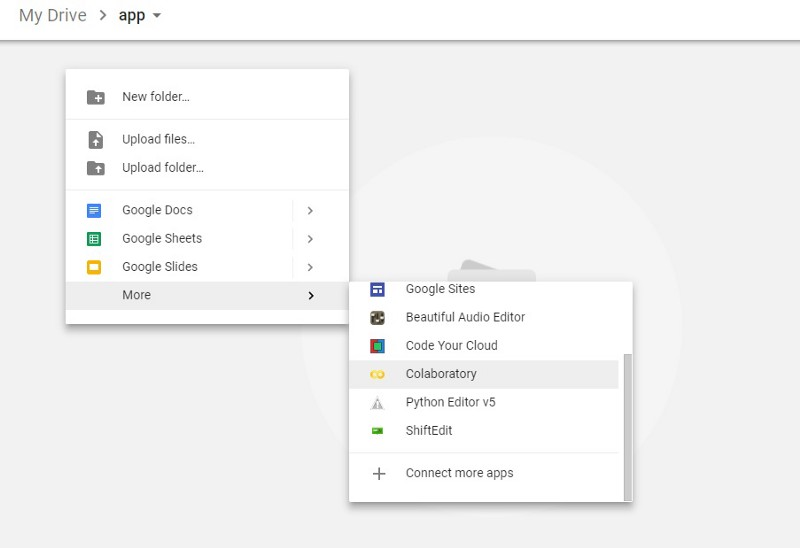
\includegraphics[width=0.8\textwidth]{colab_settings_1.jpeg}
    \label{fig:colab_settings_1}
\end{figure}

\item В разделе \textsl{Runtime->Change runtime type} выбрать GPU
\begin{figure}[h]
    \centering
    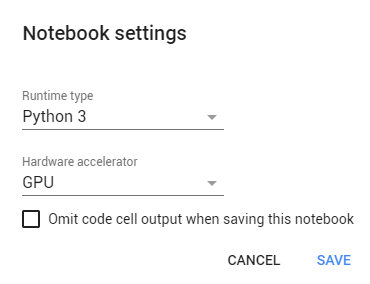
\includegraphics[width=0.6\textwidth]{colab_settings_2.png}
    \label{fig:colab_settings_2}
\end{figure}

\newpage

\item На данном этапе уже можно использовать Google Colaboratory
\begin{figure}[h]
    \centering
    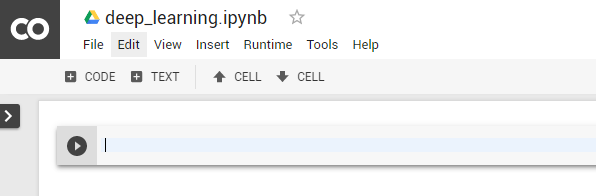
\includegraphics[width=0.85\textwidth]{colab_settings_3.png}
    \label{fig:colab_settings_3}
\end{figure}

\item Авторизуем учетную запись Google и подключим Google Drive следующими командами
\begin{figure}[h]
    \centering
    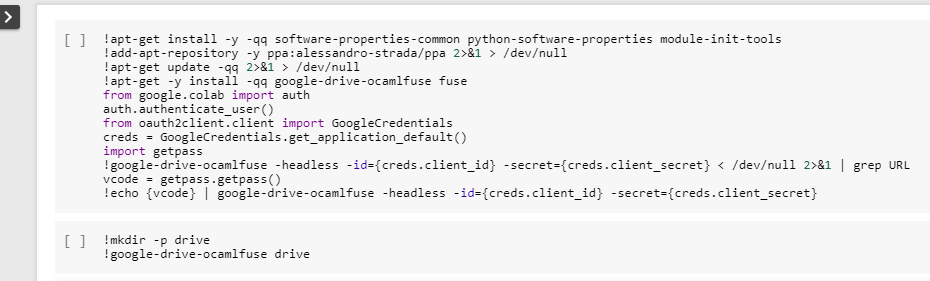
\includegraphics[width=0.85\textwidth]{colab_settings_4.png}
    \label{fig:colab_settings_4}
\end{figure}

\end{enumerate}

Теперь можно производить вычисления нa видеокарте NVIDIA Tesla K80 и взаимодействовать с Google Drive.

\newpage 

\section{Набор данных}
%\addcontentsline{toc}{section}{Набор данных}

Набор данных является одним из~важнейших объектов, лежащих в~основе обучения нейронной сети. Для~возможности обучения и проверки качества работы модели необходимо иметь репрезентативный\cite{bib:representative_data_sets} набор кодовых слов без~ошибок и с~ошибками.
Сгенерируем все информационные слова из $\mathbb{F}_2^M$. Получим множество информационных слов $A = \{a_0; a_1; \dots; a_M\}$. Элементы множества $A$ имеют следующий вид:
\begin{gather}
 % Remove numbering (before each equation)
  \nonumber a_0 = (0, 0, 0, 0, 0, 0, 0, 0, 0, 0, 0), \\
  \nonumber a_1 = (0, 0, 0, 0, 0, 0, 0, 0, 0, 0, 1), \\
  \nonumber \cdots \\
  \nonumber a_M = (1, 1, 1, 1, 1, 1, 1, 1, 1, 1, 1).
\end{gather}

Получим множество всех кодовых слов:
\begin{equation*}
  \mathbb{C} = \{a\cdot G~|~\forall a \in A \}
\end{equation*}

Получим $|\mathbb{C}| = |A| = M$. Кодовые слова кода $\mathbb{C}$ имеют следующий вид:
\begin{gather}
 % Remove numbering (before each equation)
    \nonumber c_0 = (0, 0, 0, 0, 0, 0, 0, 0, 0, 0, 0, 0, 0, 0, 0), \\
    \nonumber c_1 = (0, 0, 0, 0, 0, 0, 0, 0, 0, 0, 1, 1, 1, 1, 1), \\
    \nonumber \cdots \\
    \nonumber c_L = (1, 1, 1, 1, 1, 1, 1, 1, 1, 1, 1, 1, 1, 1, 1).
\end{gather}
\newpage
Для~генерации кодовых слов с~ошибками создадим множество масок ошибок $E = \{e_0; \dots; e_n\}.$
\begin{gather}
 % Remove numbering (before each equation)
    \nonumber e_0 = (0, 0, 0, 0, 0, 0, 0, 0, 0, 0, 0, 0, 0, 0, 0), \\
    \nonumber e_1 = (1, 0, 0, 0, 0, 0, 0, 0, 0, 0, 0, 0, 0, 0, 0), \\
    \nonumber e_2 = (0, 1, 0, 0, 0, 0, 0, 0, 0, 0, 0, 0, 0, 0, 0), \\
    \nonumber \cdots                                                \\
    \nonumber e_n = (0, 0, 0, 0, 0, 0, 0, 0, 0, 0, 0, 0, 0, 0, 1).
\end{gather}

Определим множество кодовых слов с ошибкой $\widetilde{\mathbb{C}_i}$.
\begin{equation}
  \widetilde{\mathbb{C}_i} = \{c_i \oplus e ~|~  c_i \in \mathbb{C}~\space~\forall e \in E \}, где i \in \{0; \dots; M\}
\end{equation}
где $\oplus$ - операция сложения векторов по модулю $2$. Обозначим его элементы $\widetilde{c_i}$, где $i \in \{0; \dots; n\}$ - позиция единицы в образующей маске ошибки.

Определим множество всевозможных кодовых слов с ошибкой.
\begin{equation}
  \widetilde{\mathbb{C}} = \bigcup\limits_{i=0}^{M} \widetilde{\mathbb{C}_i}
\end{equation}

Набор данных $D$ состоит из~$M$ блоков, каждый из которых состоит из $n+1$ строк и определяется случайно выбранным кодовым словом $c~\in~\mathbb{C}$.
Блок $B_i$, определяемый кодовым словом $c_i \in \mathbb{C}$, содержит множество всевозможных пар $c_i$ и соответствующих ему  слов $\widetilde{c} \in \widetilde{\mathbb{C}_i}$:
\begin{equation}
  B_i = \{ (c_i, \widetilde{c}) ~|~ \forall~\widetilde{c} \in \widetilde{\mathbb{C}_i} \}, i \in \{0; \dots; M\}
\end{equation}

Перед началом обучения нейронной сети набор данных $D$ перемешивается и сбалансированно делится на~тренировочную и валидационную выборки $D_T$ и $D_V$ соответственно в отношении 70\% к 30\%.

\newpage

Ниже приведены некоторые строки из набора данных: \\
\begin{eqnarray*}
% \nonumber % Remove numbering (before each equation)
&(0010100000100100,\>0010100000110100)& \\
&(0010100000100100,\>0010100000100000)& \\
&(0010100000100100,\>0010100010100100)& \\
&(0010100000100100,\>0010100001100100)& \\
&(0010100000100100,\>0000100000100100)& \\
&(0010100000100100,\>0010101000100100)& \\
&(0010100000100100,\>0110100000100100)& \\
&(0010100000100100,\>0010100000100110)& \\
&(0010100000100100,\>0010100000101100)& \\
&(0010100000100100,\>0010100000000100)& \\
&(0010100000100100,\>0011100000100100)& \\
&(0010100000100100,\>0010100000100100)& \\
&(0010100000100100,\>0010110000100100)& \\
&(0010100000100100,\>0010000000100100)& \\
&(0010100000100100,\>0010100100100100)& \\
&(0010100000100100,\>1010100000100100)&
\end{eqnarray*}

\newpage 

\section{Декодер на основе нейронной сети}

\subsection{Входные и выходные данные}\label{subsec:input_output}

\textbf{Входные параметры.} Нейронная сеть получает на~вход ошибочное кодовое слово $\widetilde{c} \in \widetilde{C}$,
где $\widetilde{c} = c \oplus e_j, c \in C, j \in \{1;\dots; n\}$,
представленное в~виде набора признаков $f = (f_1, \dots, f_n)$, где~$f_i$ равен значению $i$-го бита~$\widetilde{c}$.

\textbf{Пример.}
\begin{equation}
    \nonumber\widetilde{c} = (0, 0, 1, 0, 1, 0, 1, 0, 1, 1, 1, 1, 1, 1, 1)
\end{equation}
\begin{eqnarray}
 % Remove numbering (before each equation)
    \nonumber f_1 &=& 0, \\
    \nonumber f_2 &=& 0, \\
    \nonumber f_3 &=& 1, \\
    \nonumber &\cdots& \\
    \nonumber f_{15} &=& 1.
\end{eqnarray}

\textbf{Выходные параметры.} Предполагается, что на выходе будет получено слово $\hat{c}$, с некоторой вероятностью равное слову $c$.
Слово $\hat{c}$ представляется вектором вероятностей~$p$. Каждый элемент $p_i~(\in [0, 1], i \in \{1;\dots; n\})$ вектора $p$, определяет вероятность того, что на~$i$-ой позиции слова $\hat{c}$ находится бит, равный единице.

\textbf{Пример.} \\
Пусть дан вектор $p$.
$$p = (0.0, 0.1, 0.2, 0.3, 0.4, 0.49, 0.5, 0.51, 0.6, 0.7, 0.8, 0.9, 1.0, 0.5, 1.0, 1.0)$$
Тогда он определяет следующий вектор $\hat{c}$.
$$\hat{c} = (0, 0, 0, 0, 0, 0, 0, 1, 1, 1, 1, 1, 1, 0, 1, 1).$$

Далее, согласно алгоритму, описанному в разделе~\ref{subsec:neural_network}, вычисляются значение функции потерь $f_{loss}$
и обновляются веса скрытых слоев $W_i$, где $i\in\{1;\dots; S\}$.


\subsection{Функции потерь}\label{subsec:losses}

\begin{definition}
  Функция потерь $f_{loss}(y, \hat{y})$ --- функция, характеризующая величину отклонения ответа $y$ нейронной сети от правильного ответа~$\hat{y}$.
\end{definition}

Целью обучения нейронной обучения является минимизация функции потерь. Основным методом такой минимизации является градиентный спуск\cite[с.\,151]{bib:neural_networks2}.

Под цели задачи подходят следующие функции в качестве функции потерь:
\begin{eqnarray}
% \nonumber % Remove numbering (before each equation)
  \nonumber f_{log}(y, \hat{y}) &=& -\log(1 - |y-\hat{y}|), \\
  \nonumber f_{exp}(y, \hat{y}) &=& e^{|y-\hat{y}|} - 1.
\end{eqnarray}

Ниже представлены графики этих функций и их реализации\cite[раздел backend]{bib:keras} на языке Python.
\begin{figure}[h]
\center
\begin{tikzpicture}
\begin{axis}[
    axis lines = left,
    xlabel = $x$,
    ylabel = {$f(x)$},
    width = 13cm,
    height = 8cm,
    xmin = 0,
    ymax = 5,
    legend pos=south east
]
%Below the red parabola is defined
\addplot [
    domain=-0.2:2.1,
    samples=100,
    color=red
]
{-ln(1-x)};
\addlegendentry{$f_{log}$}
%Here the blue parabloa is defined
\addplot [
    domain=-0.2:2.1,
    samples=100,
    color=blue
    ]
    {e^x -1};
\addlegendentry{$f_{exp}$}
\addplot [dashed] coordinates {(1, 0) (1, 6)};

\end{axis}
\end{tikzpicture}
\caption{Графики функций потерь}\label{fig:custom_losses}
\end{figure}

\begin{figure}[h]
    \centering
    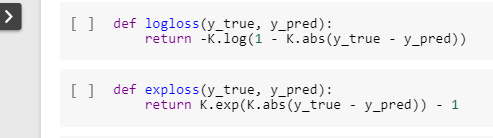
\includegraphics[width=0.9\textwidth]{losses_python.png}
    \caption{Реализации функций потерь}\label{fig:custom_losses}
    \label{fig:losses_python}
\end{figure}
\newpage
%\lstinputlisting[language=Python]{logloss_exploss.py}


\subsection{Гиперпараметры}\label{subsec:hyperparameters}

\begin{definition}
  Гиперпараметры - это такие параметры нейронной сети, которые не изменяются в~процессе обучения нейронной сети, но от~выбора которых зависит последующее качество работы сети.
\end{definition}

Определим следующий список гиперпараметров.
\begin{itemize}
  \item Количество эпох обучения $\mathbb{\varepsilon}$ нейронной сети,
  \item Количество слоев $L \in \mathbb{N}$ нейронной сети,
  \item Количество нейронов $K_i \in \mathbb{N}$ в каждом слое $l_i, i \in [1, L]$,
  \item Функция активации\cite[раздел activations]{bib:keras} нейронов $f_{a,i}: \mathbb{R} \rightarrow \mathbb{R}$ в каждом слое $l_i, i \in [1, L]$ ,
  \item Размер батча $Z \in \mathbb{N}$ [ссылка],
  \item Функция потерь\cite[раздел losses]{bib:keras} $f_{loss}$.
\end{itemize}

Для достижения максимально высокого качества работы сети необходимо найти оптимальный набор значений гиперпараметров.
Для поиска таких параметров используется библиотека hyperopt\cite{bib:hyperopt} для языка Python.
Она содержит набор функций, удобных для поиска наилучшего набора гиперпараметров.
\newpage
Определим множества значений гиперпараметров, среди которых будет осуществляться выбор.
\begin{equation}\label{eq:hyper1}
  \mathbb{\varepsilon} \in [10, 10000]
\end{equation}

\begin{equation}\label{eq:hyper1}
  L \in \{3; 4; 5; 6; 7\}
\end{equation}

\begin{equation}\label{eq:hyper2}
  K_i \in \{64; 128; 256; 512; 1024; 2048\}, где i \in \{1; \dots; L\}
\end{equation}

\begin{equation}\label{eq:hyper3}
  Z \in \{8; 16; 32; 64; 128; 256; 512\}
\end{equation}

\begin{equation}\label{eq:hyper4}
  f_{a,i} \in \{f_{relu}; f_{tanh}; f_{softmax}; f_{sigmoid}; f_{softplus}; f_{elu}\}, i \in \{1; \dots; L\}
\end{equation}

\begin{equation}\label{eq:hyper4}
  f_{loss} \in \{f_{mse}; f_{mae}; f_{binary\_crossentropy}; f_{log}; f_{exp}\}
\end{equation}

Таким образом, декартово произведение множеств значений гиперпараметров образует пространство $\mathbb{S}$.
%Adam - Оптимизация параметров производится методом стохастического градиентного спуска по дискретному множеству параметров. При этом на каждом шаге производится обучение нейронной сети и фиксация результатов.

%С ее помощью был выбран набор, определяющий количество слоев и нейронов в каждом из них, функции активации, оптимизатор, функцию потерь, размер батча и количество эпох.
\newpage 

%\subsection{Выбор оптимальных гиперпараметров}\label{subsec:opt_hyper}

Для выбора лучшего набора гиперпараметров из~пространства $\mathbb{S}$ используем функцию fmin\cite[раздел FMin]{bib:hyperopt} из~библиотеки hyperopt.
Она перебирает наборы $s \in \mathbb{S}$, для~каждого из~них строит нейронную сеть $\mathcal{N}$, обучает~ее
и сохраняет результат проверки $r$ на валидационной выборке $D_V$ и историю\cite[раздел callbacks]{bib:keras} обучения $h$.
В~процессе поиска обнаружено, что нейронные сети, содержащие функции активации  $f_a \in \{relu; elu\}$, функции потерь $f_{loss} \in \{f_{mse}; f_{mae}; f_{binary\_crossentropy}\}$, количества нейронов $K_i \in \{512; 1024; 2048\}$ и с~количеством эпох, меньшим~$1000$, показывают низкое качество.

Произведем поиск гиперпараметров в подпространстве $\hat{S} \subset \mathbb{S}$, исключающем вышеперечисленные параметры.
В~результате получим список наборов гиперпараметров $\widehat{s} = (\widehat{s}_1, \widehat{s}_2, \dots, \widehat{s}_{|\hat{S}|})$ с результатами их проверок $r_i$,
где $\widehat{s}_i \in \hat{S}$~-~набор гиперпараметров, $i \in \{1; \dots; |\hat{S}|$\}.

В результате анализа полученного списка выявлено, что наилучшее качество достигается при следующем наборе гиперпараметров:
\begin{equation}\label{eq:hyper_set}
    s^* =
    \begin{cases}
        S = 5, \\
        f_{loss} = f_{exp}, \\
        K_i \approx 208, \\
        f_{a,i}\,-\, sigmoid,\\
        Z = 256.
    \end{cases}
\end{equation}


\newpage 



\newpage 

\section{Результаты}

\subsection{Выбор оптимальных гиперпараметров}\label{subsec:opt_hyper}

Для выбора лучшего набора гиперпараметров из~пространства $\mathbb{S}$ используем функцию fmin\cite[раздел FMin]{bib:hyperopt} из~библиотеки hyperopt.
Она перебирает наборы $s \in \mathbb{S}$, для~каждого из~них строит нейронную сеть $\mathcal{N}$, обучает~ее
и сохраняет результат проверки $r$ на валидационной выборке $D_V$ и историю\cite[раздел callbacks]{bib:keras} обучения $h$.
В~процессе поиска обнаружено, что нейронные сети, содержащие функции активации  $f_a \in \{relu; elu\}$, функции потерь $f_{loss} \in \{f_{mse}; f_{mae}; f_{binary\_crossentropy}\}$, количества нейронов $K_i \in \{512; 1024; 2048\}$ и с~количеством эпох, меньшим~$1000$, показывают низкое качество.

Произведем поиск гиперпараметров в подпространстве $\hat{S} \subset \mathbb{S}$, исключающем вышеперечисленные параметры.
В~результате получим список наборов гиперпараметров $\widehat{s} = (\widehat{s}_1, \widehat{s}_2, \dots, \widehat{s}_{|\hat{S}|})$ с результатами их проверок $r_i$,
где $\widehat{s}_i \in \hat{S}$~-~набор гиперпараметров, $i \in \{1; \dots; |\hat{S}|$\}.

В результате анализа полученного списка выявлено, что наилучшее качество достигается при следующем наборе гиперпараметров:
\begin{equation}\label{eq:hyper_set}
    s^* =
    \begin{cases}
        S = 5, \\
        f_{loss} = f_{exp}, \\
        K_i \approx 208, \\
        f_{a,i}\,-\, sigmoid,\\
        Z = 256.
    \end{cases}
\end{equation}


\newpage 

\subsection{Параметры декодера}\label{subsec:arch}

Для достижения максимального качества работы декодера выполнен поиск оптимальных гиперпараметров. Проведен анализ результатов поиска и выбран набор параметров $s^*$, определенный в \ref{subsec:opt_hyper}.

Ниже представлен пошаговый процесс реализации нейронной сети $\mathcal{N}$ с параметрами $s^*$.

\begin{figure}[h]
    \centering
    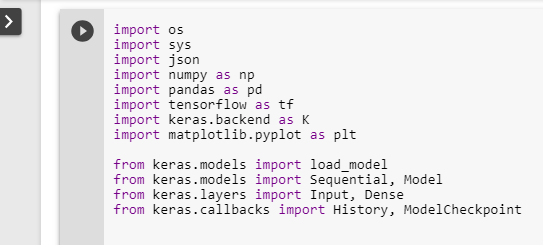
\includegraphics[width=0.9\textwidth]{neural_network_import.png}
    \caption{Импорт необходимых библиотек.}
    \label{fig:neural_network_import}
\end{figure}

\begin{figure}[h]
    \centering
    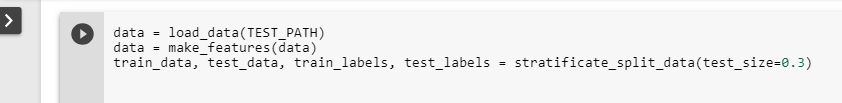
\includegraphics[width=0.9\textwidth]{neural_network_load.png}
    \caption{Загрузка и разделение данных.}
    \label{fig:neural_network_import}
\end{figure}


\begin{figure}[h]
    \centering
    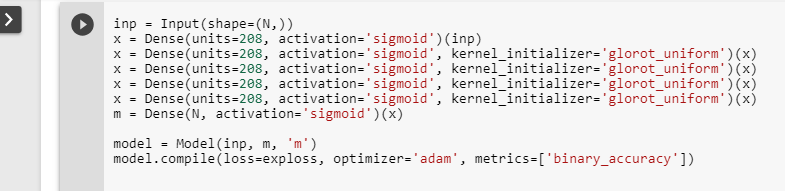
\includegraphics[width=0.9\textwidth]{neural_network_create.png}
    \caption{Создание модели нейронной сети.}
    \label{fig:neural_network_create}
\end{figure}

\newpage

\begin{figure}[h]
    \centering
    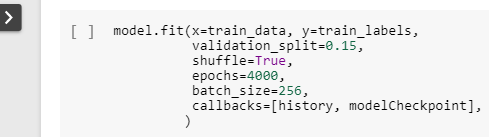
\includegraphics[width=0.9\textwidth]{neural_network_fit.png}
    \caption{Обучение модели.}
    \label{fig:neural_network_fir}
\end{figure}


\subsection{Графики обучения}\label{subsec:learning_figures}

\begin{figure}[h]
    \centering
    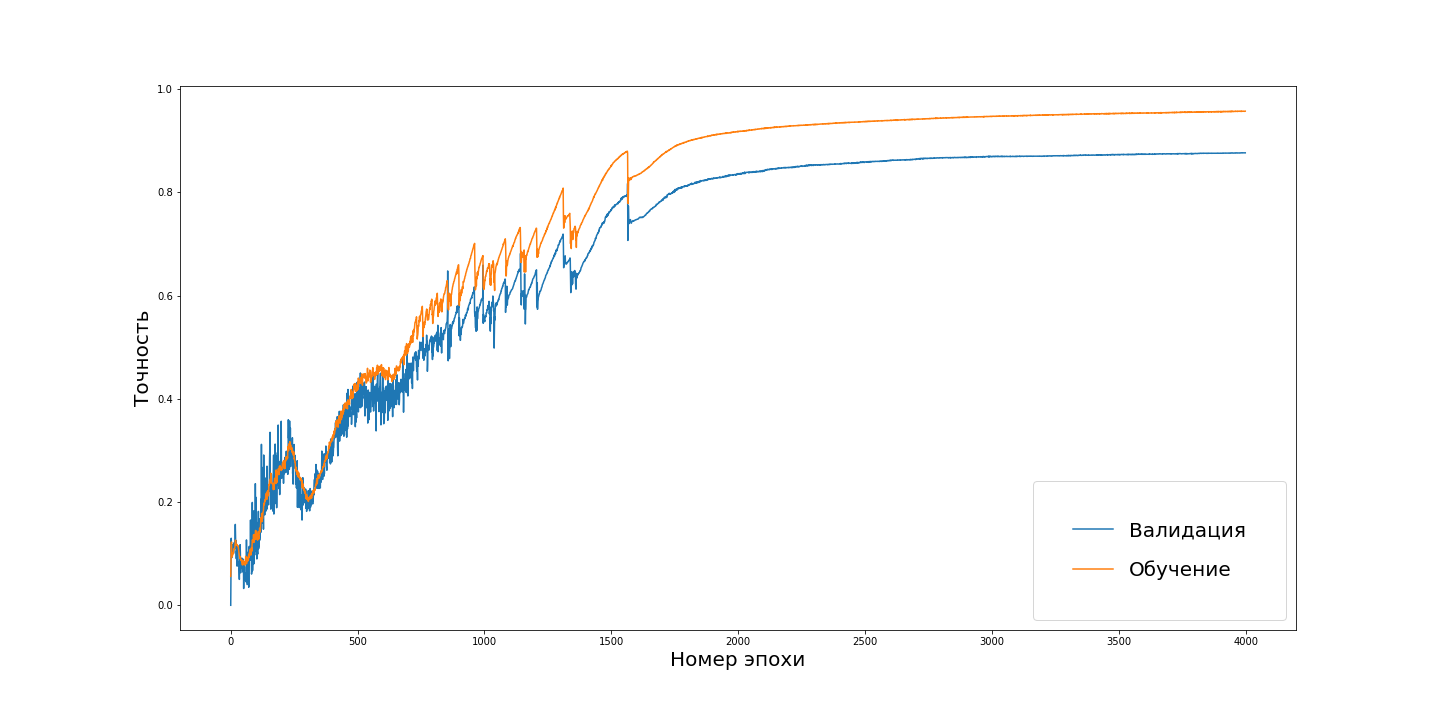
\includegraphics[scale=0.4]{model_accuracy}
    \caption{Точность модели}
    \label{fig:accuracy}
\end{figure}

\begin{figure}[h]
    \centering
    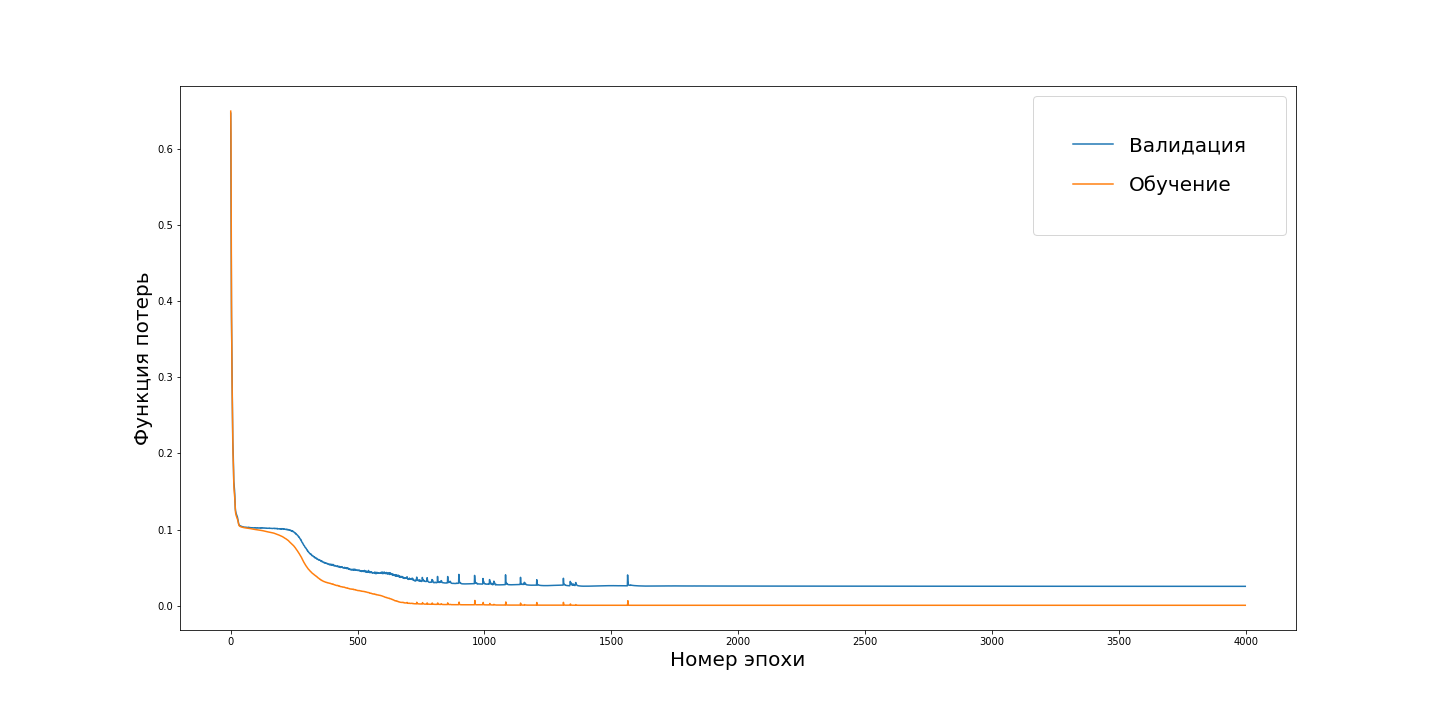
\includegraphics[scale=0.4]{model_loss}
    \caption{Функция потерь модели}
    \label{fig:loss}
\end{figure}

\newpage


\subsection{Качество работы декодера}\label{subsec:accuracy}

Определим функцию $eq$, принимающую некоторый вектор $a$ и некоторый вектор $b$ такие, что $|a|~=~|b|$:
\begin{equation}\label{eq:equal}
    eq(a, b) =
    \begin{cases}
        1, & \mbox{если } a~=~b, \\
        0, & \mbox{иначе}.
    \end{cases}
\end{equation}

Определим функцию $A(\mathcal{N}, D_V)$:
\begin{equation}\label{eq:accuracy}
    A(\mathcal{N}, D_V) = \frac{\sum\limits_{(c, \widetilde{c})\in D_V}eq(\mathcal{N}(\widetilde{c}), c)}{|D_V|}
\end{equation}

Проверка качества работы нейронной сети $\mathcal{N}$ на валидационной выборке $D_V$ осуществляется посредством функции $A$. Для нейронной сети $\mathcal{N}$ с параметрами $s^*$:
\begin{equation}\label{eq:final_accuracy}
  A(\mathcal{N}_{s^*}, D_V)~\approx~0.92.
\end{equation}

Таким образом, получен декодер помехоустойчивого кода на основе нейронной сети с вероятностью исправления одной ошибки, равной $92 \%$.

\newpage 


\section{Заключение}\label{subsec:conclusions}

В данной работе представлена реализация нейронной сети $\mathcal{N}$, позволяющей выполнять декодирование кода Хэмминга с использованием технологии Google Colaboratory. В разделе~\ref{subsec:accuracy} показано, что нейронная сеть~$\mathcal{N}$ с~точностью 0.92 исправляет одну ошибку в кодовом слове. Таким образом, поставленные цели достигнуты.

Полученный в ходе работы результат имеет исследовательский характер и показывает, что идея использования нейронных сетей в задачах декодирования помехоустойчивых кодов является оправданной. В дальнейших исследованиях представляется возможным исследовать приминимость нейронных сетей для декодирования других, более сложных, кодов. Такие исследования являются социально полезными, так как сферы применения кодов крайне обширны.

\newpage


\section{Список литературы}

\bibliographystyle{utf8gost705u}  %% стилевой файл для оформления по ГОСТу
\bibliography{bibliography}     %% имя библиографической базы (bib-файла)


\end{document}























